\graphicspath{{chapters/15/images}}
\chapter{Protein motions}

\section{Elastic network models (ENM)}

\begin{figure}[H]
	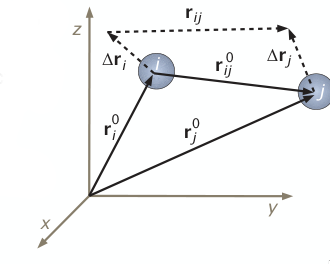
\includegraphics[width=\textwidth]{enm-theory}
	\caption{Elastic network models}
	\label{fig:kirchhoff-adjacency}
\end{figure}

Configuration vector of the protein: $\vec{r} = [\vec{r}_1, \vec{r}_2, \dots, \vec{r}_N]$.
Deviation from the equilibrium position (PDB structure):

$$\Delta\vec{r}_i = \vec{r}_i-\vec{r}_i^0$$

Instantaneous changes in the positions of all residues:

$$\Delta\vec{r} = [\Delta\vec{r}_1, \Delta\vec{r}_2, \dots, \Delta\vec{r}_N]$$


Equilibrium separation between two beads $i$ and $j$: $\vec{r}_{ij}^0 = \vec{r}_j^0-\vec{r}_i^0$.
Instantaneous separation between two beads $i$ and $j$: $\vec{r}_{ij} = \vec{r}_{ij}^0+\Delta\vec{r}_{ij}$, $\Delta\vec{r}_{ij} = \Delta\vec{r}_i-\Delta\vec{r}_i$.

\section{Gaussian network model (GNM)}
Potential energy for each couple:

$$U_{ij} = \gamma_{ij}(\Delta\vec{r}_j-\Delta\vec{r}_i)\cdot(\Delta\vec{r}_j-\Delta\vec{r}_i) = \gamma_{ij}\Delta\vec{r}_{ij}^2$$

Total elastic energy:

$$U_{GNM} = \frac{1}{2}\sum\limits_i\sum\limits_j\gamma_{ij}\Delta\vec{r}^2_{ij} = \frac{\gamma}{2}\sum\limits_i\sum\limits_j\Delta\vec{r}_{ij}^2$$

Cutoff radius: $r_c = \si{\angstrom}$.

So the total potential energy:

$$U_{GNM} = \frac{\gamma}{2}\Delta\vec{r}(t)^T\Gamma\Delta\vec{r}(t)$$

Where $\Gamma$ is the Kirchoff adjacency matrix.

\begin{figure}[H]
	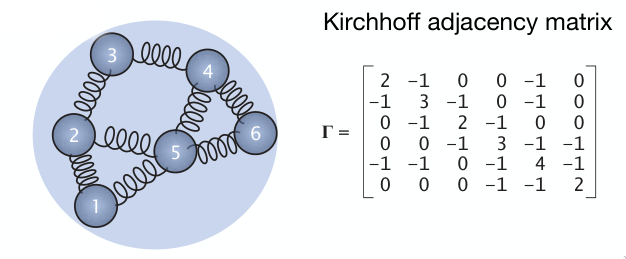
\includegraphics[width=\textwidth]{kirchoff-adjacency-matrix}
	\caption{Kirchhoff adjacency matrix}
	\label{fig:kirchhoff-adjacency}
\end{figure}

	\subsection{Correlated motions}

	$$\langle\Delta\vec{r}_i\cdot\Delta\vec{r}_j\rangle = \frac{1}{Q}\int\Delta\vec{r}_i\cdot\Delta\vec{r}_je^{-\frac{U}{kT}}d^N\Delta\vec{r}$$

	Generalized Gaussian integral:

	$$\langle\Delta\vec{r}_i\cdot\Delta\vec{r}_j\rangle = \frac{3kT}{\gamma}[\Gamma^{-1}]_{ij}$$

	Where $\Gamma^{-1}$ is a pseudoinverse matrix as the Kirchhoff matrix has zero determinant and cannot be inverted.
	Considering the eigenvalue decomposition: $\Gamma = U\Lambda U^T$:

	$$U = [\vec{u}_1, \dots, \vec{u}_{N_1}] = \begin{bmatrix} u_{1,1} & \cdots & u_{N-1,1}\\\vdots & \cdots & \vdots\\ u_{1, N} & \cdots & u_{N-1, N}\end{bmatrix}\qquad\Lambda = \begin{bmatrix} \lambda_1 & 0 & 0 & \cdots & 0\\ 0 & \lambda_2 & 0 &\cdots & 0\\0 & 0& \lambda_3 & \cdots & 0\\\vdots & \vdots & \vdots & \vdots &\vdots\\ 0 & 0 & 0 & \cdots & \lambda_{N-1}\end{bmatrix}$$

	\subsection{Gaussian network model and B-factors}

	$$\langle\Delta\vec{r}_i\cdot\Delta\vec{r}_i\rangle = \frac{3kT}{\gamma}[U\Lambda^{-1}U^{T}]_{ii} = \frac{3kT}{\gamma}\sum\limits_{k}[\lambda_k^{-1}\vec{u}_k\vec{u}_k^T]_{ii} = \sum\limits_{k}[\Delta r_i^2]_k$$

	Debye-Waller factors:

	$$B_i = \frac{8\pi^2}{3}\langle\Delta r_i^2\rangle$$

	\begin{figure}[H]
		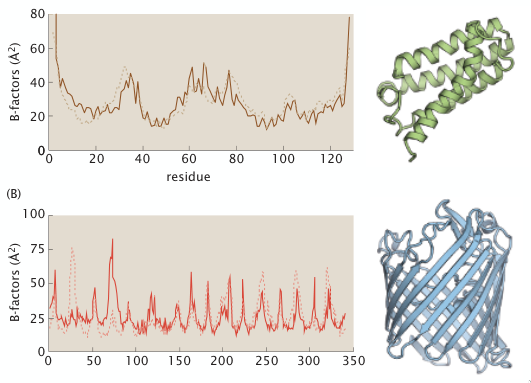
\includegraphics[width=\textwidth]{gnm-b-factors}
		\caption{GNM and B-factors}
		\label{fig:gnn-b-factors}
	\end{figure}

	\subsection{Biological relevance}

	\begin{figure}[H]
		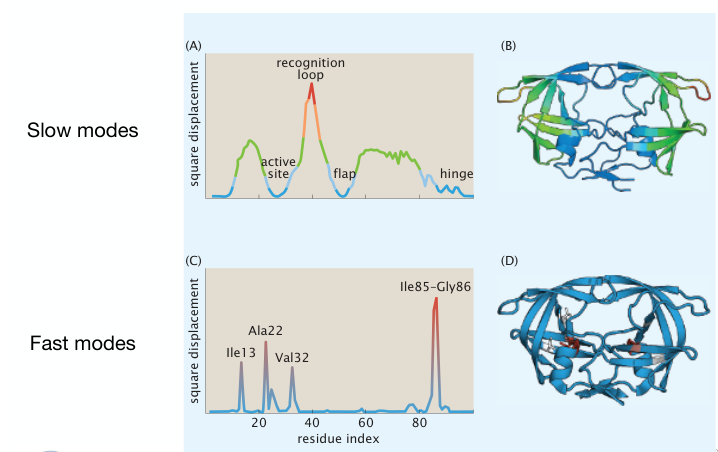
\includegraphics[width=\textwidth]{biological-relevance}
		\caption{Biological relevance}
		\label{fig:biological-relevance}
	\end{figure}

	\subsection{Normal mode analysis}

	$$U = U_0 + \sum\limits_i\frac{\partial U}{\partial q_i}|_{q^0}(q_i-q_i^0) + \frac{1}{2}\sum\limits_i\sum\limits_j\frac{\partial^2 U}{\partial q_i\partial q_j}|_{q^0}(q_i-q_i^0)(q_j-q_j^0) + \cdots$$

	At equilibrium:

	$$U = \frac{1}{2}\Delta\vec{q}^TH\Delta\vec{q} = \frac{1}{2}\sum\limits_i\sum\limits_j H_{ij}(q_i-q_i^0)(q_j-q_j^0)$$

	Hessian matrix:

	$$H_{ij} = \frac{\partial^2 U}{\partial q_i\partial q_j}|_{q^0}$$

	Covariance matrix:

	$$C = \langle\Delta\vec{q}\Delta\vec{q}^T\rangle = \frac{1}{Q}\int\Delta\vec{q}\Delta\vec{q}^Te^{-\frac{\Delta\vec{q}^TH\Delta\vec{q}}{2kT}}d^N\Delta\vec{q} = kTH^{-1}$$

\section{Anisotropic network model (ANM)}

$$U_{ANM} = \frac{1}{2}\sum\limits_{ij}\gamma(r_{ij}-r_{ij}^0)^2\Rightarrow\frac{\partial^2 U}{\partial x_i\partial y)i} = -\gamma\frac{(x_i-x_i)(y_i-y_j)}{t_{ij}^2}$$

Hessian matrix:

$$H_{ij} = \frac{\gamma}{r_{ij}^2}\begin{bmatrix}x_{ij}^2 & x_{ij}y_{ij} & x_{ij}z_{ij}\\x_{ij}y_{ij} & y_{ij}^2 & y_{ij}z_{ij}\\ x_{ij}z_{ij} & y_{ij}z_{ij} & z_{ij}^2\end{bmatrix}$$

Eigenvalue decomposition: $H=U\Lambda U^T$:

$$\Lambda = \begin{bmatrix}\lambda_1 & 0 & 0 & \cdots & 0\\ 0 & \lambda_2 & 0 & \cdots & 0\\ 0 & 0 & \lambda_3 & \cdots & 0\\\vdots & \vdots & \vdots & \vdots & \vdots\\ 0 & 0 & 0 & \cdots & \lambda_{3N-6}\end{bmatrix}$$

	\subsection{Correlated motions}

	$$\langle\Delta\vec{r}_i\cdot\Delta\vec{r}_j\rangle = \frac{3kT}{\gamma}[U\Lambda^{-1}U^T]_{ij} = \frac{3kT}{\gamma}\sum\limits_{k}\lambda_k^{-1}[\vec{u}_k\vec{u}_k^T]_[ij]$$

	\begin{figure}[H]
		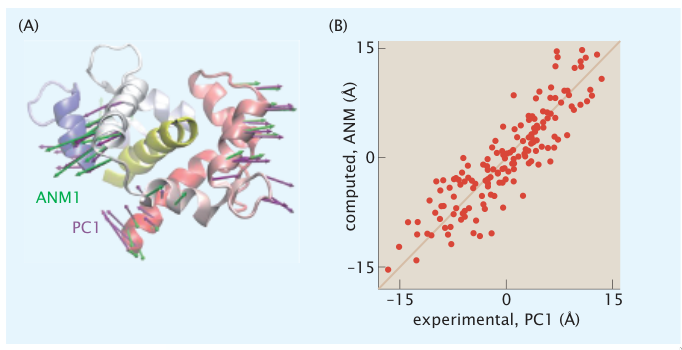
\includegraphics[width=\textwidth]{asm-correlated-motion}
		\caption{Correlated motions}
		\label{fig:as-correlated-motion}
	\end{figure}

	Correlated cosine:

	$$I_k = \frac{\Delta\vec{q}_{AB}\cdot\vec{u}_k}{|\Delta\vec{q}_{AB}|}\qquad \Delta\vec{q}_{AB} = \vec{q}^B-\vec{q}^A$$

	Cumulative overlap:

	$$C_0 = \sqrt{\sum\limits_k I_k^2}$$

	Degree of collectivity:

	$$\kappa_k = N^{-1}e^{-\sum\limits_{i=1}^N\alpha(\Delta r_i)^2|_k\log(\alpha\Delta r_i)^2|_k}$$

	$$\sum\limits_{i=1}^N\alpha(\Delta r_1)^2|_k = 1$$

\section{Essential dynamics}

\begin{enumerate}
	\item Obtain trajectories from molecular dynamics simulations, better if equilibrated.
	\item Remove overall translations and rotations by aligning each frame to a reference structure.
	\item Choose the set of atoms for the analysis like $\alpha$-carbons.
	\item Obtain the covariance matrix:

		$$C_{ij} = (x_i(t) - \bar{x_i(t)})(x_j(t)-\bar{x_j(t)})$$

	\item If the fluctuations display some non-homogeneous behaviour, it is better to employ the correlation matrix:

		$$R_{ij} = \frac{(x_i(t)-\bar{x_i(t)})(x_j(t)-\bar{x_j(t)})}{\sigma_{x_i}\sigma_{x_j}}$$

	\item Diagonalize $C$ or $R$ employing eigenvalue decomposition EVD as in elastic network models.
	\item Examine the eigenvalue scree plot to determine the number of eigenvectors to include in the reduced vector space that describes the most relevant features.

	\begin{figure}[H]
		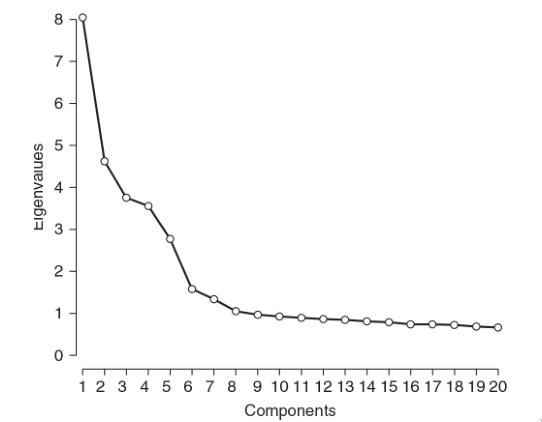
\includegraphics[width=\textwidth]{eigenvalue-scree-plot}
		\caption{Eigenvalue scree plot}
		\label{fig:eigenvalue-scree-plot}
	\end{figure}

\item Select the top set of eigenvectors to form the PCs (usually between $2$ an $20$).
\item Examine the eigenvector collectivity defined as in the ANM: top modes tend to be more collective than lower modes, indicating that many residues are participating in collective motions.

	\begin{figure}[H]
		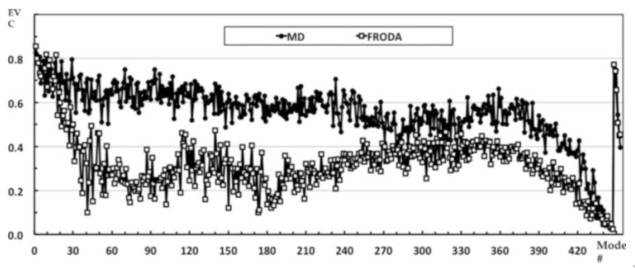
\includegraphics[width=\textwidth]{eigenvalue-collectivity}
		\caption{Eigenvalue collectivity}
		\label{fig:eigenvalue-collectivity}
	\end{figure}

\item Construct the weighted RMSD modes $\langle\Delta\vec{r}_i^2\rangle_k = \lambda_k[\vec{u}_k\vec{u}_k^T]_{ij}$.
	Visualize which residues contribute most to the fluctuation of each PCA mode.

	\begin{figure}[H]
		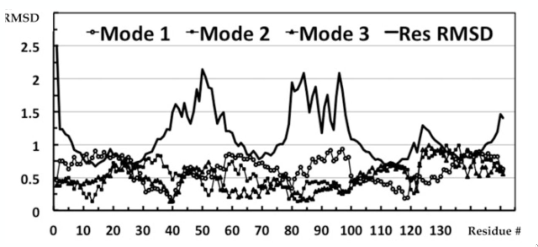
\includegraphics[width=\textwidth]{weighted-rmsd}
		\caption{Weighted RMSD modes}
		\label{fig:weighted-rmsd}
	\end{figure}

\item Construct the displacement vectors $\vec{d}_i(t) = \vec{r}_i(t)-\bar{\vec{r}_i}$ for each snapshot and construct the PCs:

	$$PC_k(t) = \sum\limits_{i=1}^N\vec{d}_i(t)\cdot\vec{u}_i^k\qquad\text{ with }k=1, \dots, 3N-6$$

	\begin{figure}[H]
		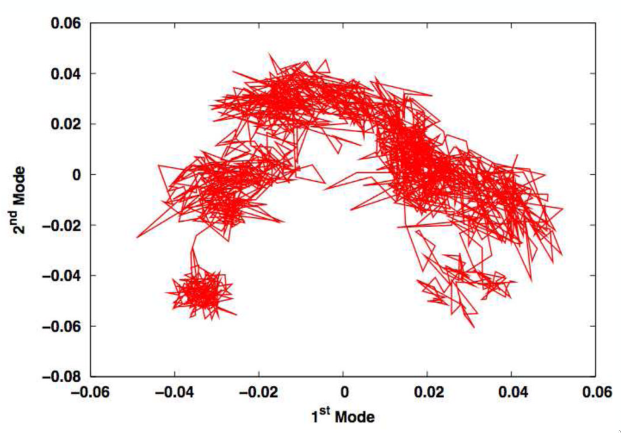
\includegraphics[width=\textwidth]{scatter-plot-pcs-modes}
		\caption{Scatter plot of first and second mode for PCs}
		\label{fig:scatter-plot-pcs-modes}
	\end{figure}

	\begin{figure}[H]
		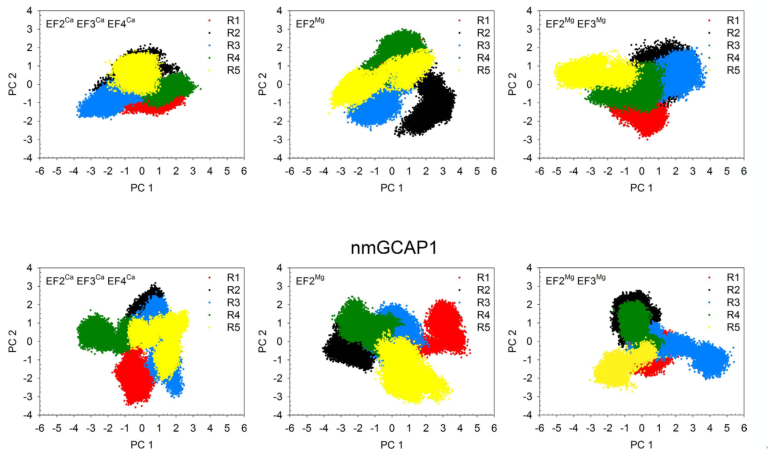
\includegraphics[width=\textwidth]{scatter-plot-pcs}
		\caption{Scatter plot of PCs}
		\label{fig:scatter-plot-pcs}
	\end{figure}

\item Examine the cosine content for each mode $k$, defined as the superposition with the cosine obtained from a simple diffusion in a high dimensional harmonic potential:

	$$c_k = \frac{2}{T_{sim}}\biggl(\int_0^{T_{sim}}\cos\biggl(\pi\frac{k_BT}{\lambda_k}t\biggr)PC_k(t)dt\biggr)^2\biggl(\int_0^{T_{sim}}PC_k^2(t)dt\biggr)^{-1}$$

	\begin{figure}[H]
		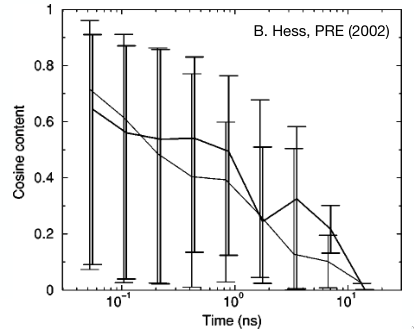
\includegraphics[width=\textwidth]{cosine-content}
		\caption{Cosine content for the modes}
		\label{fig:cosine-content}
	\end{figure}

\item Examine the similarity between trajectories or between portions of the same trajectory by examining the Covariance overlap:

	$$\Omega_{A, B} = 1 - \biggl[\frac{\sum\limits_{k=1}^{3N-6}(\lambda_k^A+\lambda_k^B)-2\sum\limits_{k=1}^{3N-6}\sum\limits_{j=1}^{3N-6}\sqrt{\lambda_k^A\lambda_j^B}(\vec{u}_k^A\cdot\vec{u}_j^B)^2}{\sum\limits_{k=1}^{3N-6}(\lambda_k^A+\lambda_k^B)}\biggr]^{\frac{1}{2}}$$

	$\Omega_{A, B} = 1$ if and only if the two covariance matrices are identical, while it is zero when the sampled subspaces are completely orthogonal.
\end{enumerate}
